% Journal version in the format of the IEEE Transactions on Consumer Electronics (IEEEtran journal): the same
% sections as access.tex (sections/access_*.tex). TCE allows 8 pages without overlength charges (2026 IEEE APC list).
% Every number comes from tables/numbers.tex or tables/tab_*.tex (paper/make_assets.py). Never type results.
\documentclass[journal]{IEEEtran}
\IEEEoverridecommandlockouts
% Shared by conference.tex (IEEEtran, 6 pages) and access.tex (IEEE Access, full length).
% Every number in either paper comes from tables/numbers.tex or tables/tab_*.tex, which
% paper/make_assets.py generates from paper/data/. Do not type results by hand.
\usepackage{cite}
\usepackage{amsmath,amssymb}
\usepackage{graphicx}
\usepackage{booktabs}
\usepackage{xcolor}
\usepackage{tikz}
\usetikzlibrary{arrows.meta,positioning,fit,calc,backgrounds,shapes.geometric,decorations.pathreplacing}
\usepackage[siunitx,american]{circuitikz}
% Shared TikZ styles for the hand-drawn architecture and circuit figures (paper/figures/tikz/*.tex).
% Both papers load this file; every figure here is drawn from the RTL (rtl/*.v) and the block design
% (future_work/board/block_design.tcl) it depicts, so keep them in sync when either changes.
\definecolor{psfill}{RGB}{226,236,250}
\definecolor{plfill}{RGB}{252,236,218}
\definecolor{cryfill}{RGB}{250,214,214}
\definecolor{netfill}{RGB}{236,236,236}
\definecolor{rxfill}{RGB}{222,242,226}
\definecolor{inkc}{RGB}{40,40,40}
\tikzset{
  blk/.style={draw=inkc, rounded corners=1pt, minimum height=6mm, align=center, inner sep=2pt, font=\scriptsize, fill=white},
  cry/.style={blk, fill=cryfill},
  arm/.style={blk, fill=psfill},
  pl/.style={blk, fill=plfill},
  rx/.style={blk, fill=rxfill},
  grp/.style={draw=inkc, rounded corners=3pt, inner sep=3mm},
  arr/.style={-{Latex[length=1.5mm]}, inkc},
  darr/.style={{Latex[length=1.5mm]}-{Latex[length=1.5mm]}, inkc},
  bus/.style={-{Latex[length=1.6mm]}, line width=0.9pt, inkc},
  lbl/.style={font=\tiny, inner sep=1pt},
  ttl/.style={font=\scriptsize\bfseries, inner sep=1pt},
}

\newcommand{\TODO}[1]{\textcolor{red}{[TODO: #1]}}
% \ifextended: content only in the full-length (IEEE Access) version; the generated tables use it too
\newif\ifextended
% generated by paper/make_assets.py from paper/data -- do not edit
\newcommand{\AesGcmMs}{0.01}
\newcommand{\AllDecode}{all}
\newcommand{\BenignFalse}{0/447}
\newcommand{\BenignLatency}{82}
\newcommand{\BenignPninetyfive}{278}
\newcommand{\BenignRuns}{3}
\newcommand{\CostEfive}{31.0}
\newcommand{\CostEfour}{29.5}
\newcommand{\CostEtwo}{13.4}
\newcommand{\CryptoLutShare}{54}
\newcommand{\CyclesPerPixel}{1.64}
\newcommand{\Decoders}{Pillow, OpenCV, scikit-image, FFmpeg (MJPEG)}
\newcommand{\FbDropTtm}{3.5}
\newcommand{\FpsHD}{66}
\newcommand{\FpsVGA}{199}
\newcommand{\JigsawNeighboursMax}{1.7}
\newcommand{\JigsawOracleMax}{0.47}
\newcommand{\JigsawOracleMin}{0.41}
\newcommand{\LeakEFiveMax}{0.017}
\newcommand{\LeakEFiveMin}{-0.004}
\newcommand{\LeakEOneFourMax}{0.58}
\newcommand{\LeakEOneFourMin}{0.27}
\newcommand{\LearnEfiveEdgeMax}{0.021}
\newcommand{\LearnEpochs}{25}
\newcommand{\LearnSsimMax}{0.43}
\newcommand{\LearnTest}{400}
\newcommand{\LearnTrain}{1000}
\newcommand{\MaxExtraCycles}{5}
\newcommand{\NumAttacks}{11}
\newcommand{\NumClips}{4}
\newcommand{\NumDecoders}{4}
\newcommand{\OverheadEfiveQVGA}{12}
\newcommand{\OverheadEfiveVGA}{21}
\newcommand{\OverheadEtwoQVGA}{0.5}
\newcommand{\OverheadEtwoVGA}{0.3}
\newcommand{\PolCostB}{0.162}
\newcommand{\PolCostSave}{14}
\newcommand{\PolCostT}{0.188}
\newcommand{\PolFalse}{0/6020}
\newcommand{\PolLeakB}{0.054}
\newcommand{\PolTtmB}{1.34}
\newcommand{\PolTtmT}{0.46}
\newcommand{\PyPlainMs}{134}
\newcommand{\PySelEtwoMs}{151}
\newcommand{\RealTalkFalse}{0/125}
\newcommand{\RealTalkMit}{11/11}
\newcommand{\RealTalkTtm}{1.09}
\newcommand{\RealTrailerFalse}{0/125}
\newcommand{\RealTrailerMit}{11/11}
\newcommand{\RealTrailerTtm}{0.89}
\newcommand{\ResourceSource}{a Yosys synthesis estimate}
\newcommand{\Seeds}{10}
\newcommand{\SuiteFalse}{0/375}
\newcommand{\SuiteLatency}{97}
\newcommand{\SuiteRuns}{3}
\newcommand{\TopLutPct}{10.7}
\newcommand{\TopLuts}{5{,}681}
\newcommand{\TtmMean}{0.91}
\newcommand{\TtmSd}{0.02}
\newcommand{\TurboFps}{1047}
\newcommand{\TurboMs}{0.95}

% ---------------------------------------------------------------- notation (Section "Notation" in access.tex)
\newcommand{\xor}{\oplus}
\newcommand{\cat}{\,\|\,}
\newcommand{\Kseg}{K_{\mathrm{seg}}}
\newcommand{\Kfb}{K_{\mathrm{fb}}}
\newcommand{\Nenc}{N^{\mathrm{enc}}}
\newcommand{\Nmac}{N^{\mathrm{mac}}}
\newcommand{\Enc}{\mathcal{E}}
\newcommand{\MAC}{\mathrm{MAC}}
\newcommand{\KDF}{\mathrm{KDF}}
\newcommand{\amp}{\mathcal{A}}
\newcommand{\sz}{\mathrm{cat}}

\usepackage{amsthm}
\newtheorem{proposition}{Proposition}
\newtheorem{lemma}{Lemma}
\theoremstyle{definition}\newtheorem{definition}{Definition}
\usepackage[hidelinks]{hyperref}
\extendedtrue

\begin{document}
\title{Playable but Private: In-Encoder Selective Encryption with Ascon-AEAD128 and Attack-Adaptive Protection for MJPEG Video on an FPGA SoC}
\author{Aravind~R, Suhas~V~J, Rishab~H~R, Samarth~B~N, Vijaysurya~B~S, and~Chetana~G\,\TODO{order, IEEE membership}%
\thanks{The authors are with the Department of Electronics and Communication Engineering, RV College of Engineering, Bengaluru 560059, India \TODO{e-mails}. \TODO{funding statement, or ``This work received no external funding.''}}}
\markboth{IEEE Transactions on Consumer Electronics}{Aravind R \MakeLowercase{\textit{et al.}}: Playable but Private}
\maketitle

\begin{abstract}
Home cameras, video doorbells and baby monitors stream over networks their owners do not control, yet encrypting the whole stream makes it unplayable without the key and spends cipher work on every byte. We present a JPEG/MJPEG encoder for a Zynq-7020 FPGA SoC that encrypts the sign and amplitude bits of selected DCT coefficients inside the entropy coder, with a keystream from the NIST standard Ascon-AEAD128. We prove that the transformation never changes a Huffman code length, so every protection level is a valid JPEG that standard players and recorders accept, and a 128-bit tag over the frame metadata and the coded scan rejects any modified, replayed or forged frame. The strongest level hides block positions with a keyed, per-frame permutation of restart segments that needs no frame buffer: the fabric codes and authenticates one segment per macroblock and the processor only reorders them. On a PYNQ-Z2 board the design is bit-exact with its golden model in all six levels and adds no cycles for encryption; four lanes at \BdFourMhz\,MHz encode \BdFourBusyMpix\,Mpixel/s, exactly the cycle count of the RTL simulation, and a complete authenticated 640$\times$480 frame takes \BdFourZcMs\,ms, \BdSpeedupFrame{} times faster than the same encoder on the board's two ARM cores. Under the same keyless attacks on \BenchSources{} sources, four re-implemented published schemes leak \BenchPubMin--\BenchPubMax{} edge correlation while our permutation level stays at or below \BenchEfiveMax{}, also against jigsaw solvers, sign recovery and trained networks. An authenticated feedback loop mitigates all \NumAttacks{} modelled network attacks, in simulation and with the board as the camera, without false alarms.
\end{abstract}

\begin{IEEEkeywords}
consumer cameras, video privacy, selective encryption, MJPEG, Ascon, FPGA, authenticated encryption, hardware security
\end{IEEEkeywords}

% =====================================================================================================
\section{Introduction}\label{sec:intro}
Home cameras, video doorbells and baby monitors send video over Wi-Fi and shared networks that their owners do not control. Two properties matter for such a link. \emph{Confidentiality} keeps a bystander on the network from watching the home; \emph{integrity} lets the viewer trust that what it shows was captured by the camera and was not edited, replayed or injected on the way. Encrypting the transport with TLS, SRTP~\cite{rfc3711} or a VPN provides both, but it hides the stream from every recorder, player and cloud service outside the key infrastructure, and the cipher work grows with the full bitrate of a low-power device.

Selective encryption encrypts only the parts of the compressed stream that carry most of the picture and keeps the format~\cite{massoudi2008}, so standard decoders still parse the result. For baseline JPEG, the sign and the appended amplitude bits of the quantized DCT coefficients can be encrypted without changing any Huffman code length~\cite{vandroogenbroeck2002,auer2013}. Such schemes are easy to weaken: the positions of the non-zero coefficients stay visible, so an attacker still sees the outline of the scene~\cite{massoudi2008,lin2024,hirose2024}; most use key material that does not change from frame to frame, so one known frame exposes the next; and almost none authenticate what they encrypt.

We ask how much of a secure camera link fits into the encoder hardware, and what an eavesdropper still learns. Our contributions are:
\begin{enumerate}
\item \textit{Authenticated selective encryption inside the entropy coder.} A Verilog MJPEG encoder XORs a keystream of the NIST standard Ascon-AEAD128~\cite{sp800232,ascon} onto coefficient signs and amplitudes. We prove that every code length is preserved (Lemma~\ref{lem:format}) and that the cipher never stalls the encoder (Proposition~\ref{prop:supply}); a 128-bit tag binds the scan to the protection level, session, frame counter and size.
\item \textit{A hardware form of a keyed macroblock permutation (E5).} The fabric codes one restart segment per macroblock with its own keystream and authenticates them in raster order; the ARM core sends them in a keyed order that changes with every frame. No frame buffer is needed, and the order is authenticated.
\item \textit{Parallel lanes and a measured system.} Restart segments make lanes independent; one, two and four lanes produce identical bytes. On a PYNQ-Z2 board every image is bit-exact with the golden model in every level, and the encoding clocks counted by the fabric equal the RTL simulation's to within \BdBusyVsRtlMaxPct\,\% (four lanes: \BdFourBusyMpix\,Mpixel/s at \BdFourMhz\,MHz).
\item \textit{One benchmark for all schemes.} Six protection levels and four published format-compliant schemes~\cite{vandroogenbroeck2002,kishore2015,auer2013,hirose2024} under the same keyless attacks, including puzzle solvers, sign recovery, a chosen-plaintext attack and trained networks, on \NumVideoClips{} clips and the Kodak set.
\item \textit{A closed feedback loop.} An authenticated feedback channel, a forward-secure key ratchet and an adaptive policy raise protection when the receiver reports an attack, in simulation and with the board as the camera.
\end{enumerate}
\TODO{Once the conference version is accepted: cite it here and state what this article adds (proofs, board evaluation, full benchmark, protocol analysis).}

% =====================================================================================================
\section{Related Work}\label{sec:related}
\textit{Selective encryption of JPEG.} Van Droogenbroeck and Benedett encrypted the appended bits of AC coefficients and kept the Huffman code words~\cite{vandroogenbroeck2002}; Puech and Rodrigues encrypted selected DCT coefficients with AES in OFB mode~\cite{puech2005}; Auer et al.\ permuted code-word/value pairs and toggled value bits at bitstream level at more than 25 VGA frames per second~\cite{auer2013}. Massoudi et al.\ note that visual distortion does not measure security~\cite{massoudi2008}. The idea has been carried to H.264/AVC and HEVC~\cite{boyadjis2017}.

\textit{Attacks.} Lin et al.\ recover DCT sign bits by linear programming~\cite{lin2024}. Hirose et al.\ show that the number of non-zero coefficients per block, which no field encryption hides, rebuilds contours unless the restart segments are permuted~\cite{hirose2024}; Li et al.\ recover block shuffles from one designed plaintext~\cite{li2025shuffle}; a GAN-based ciphertext-only attack recovers content from most privacy-preserving image schemes~\cite{sirichotedumrong2020}; and block permutations invite jigsaw solvers, from greedy placement~\cite{pomeranz2011} to minimum-spanning-tree assembly~\cite{gallagher2012}.

\textit{Hardware.} Kishore et al.\ added block and symbol scrambling to an FPGA JPEG encoder at 13--17\,\% more ALUTs~\cite{kishore2015}; Ba\u{g}baba and \"Ors combined an FPGA JPEG encoder with TEA encryption of DC and low AC coefficients~\cite{bagbaba2015}; Qiu et al.\ XOR raw frames with chaotic sequences on a satellite payload~\cite{qiu2025}. None authenticates frames, and their key material is fixed. Commercial JPEG cores process one sample per clock at 150--166\,MHz without cryptography~\cite{logijpge,castjpeg}. Ascon is small in hardware, about 7\,kGE for one unrolled round, and a threshold implementation costs about 3.1 times the area of the low-area core~\cite{gross2017}; Ascon-based MACs~\cite{khairallah2023} and Ascon with replay detection~\cite{kurian2025} have been built on Artix-7. Farahmand et al.\ measure cryptographic cores on a Zynq-7020 with DMA, cycle-exact timers and bit-exact comparison with software~\cite{farahmand2016}; our board evaluation follows the same principles.

\textit{Traffic analysis.} Sizes and timing of encrypted streams reveal motion~\cite{wampler2015} and which video is played~\cite{schuster2017}; traffic shaping hides activity at a large bandwidth cost~\cite{apthorpe2019}. No content encryption changes this, so we measure it separately.

We found no design that places a standardized AEAD inside a hardware JPEG encoder, keeps every level playable while authenticating each frame, hides block positions without a frame buffer, and closes the loop from the receiver back to the encoder.

% =====================================================================================================
\section{Background and Threat Model}\label{sec:background}
\textit{Baseline JPEG.} Pixels are converted to YCbCr 4:2:0, so a 16$\times$16 macroblock (MCU) yields six 8$\times$8 blocks, or 1.5 samples per pixel. Each block is transformed by an integer DCT and quantized; the 64 coefficients are read in zig-zag order. The DC coefficient is coded as the difference to the previous block of its component, and each non-zero AC coefficient as a Huffman code for the pair (run of zeros, size category $s$) followed by an $s$-bit appended field~\cite{t81,wallace1992}. For $v \ne 0$,
\begin{equation}
s(v) = \lfloor \log_2 |v| \rfloor + 1, \qquad
\amp(v) = \begin{cases} v, & v > 0,\\ v + 2^s - 1, & v < 0. \end{cases}
\label{eq:amp}
\end{equation}
Two properties follow, and the design rests on both: the field can be changed without changing the Huffman code or the stream length as long as $s$ is kept, and the run lengths and size categories, i.e.\ where the non-zero coefficients are, stay visible to anyone. A restart marker ends a restart segment: the bits are padded to a byte, the DC predictors reset, and the next segment decodes without the previous one~\cite{t81}.

\textit{Ascon-AEAD128.} Ascon~\cite{ascon,sp800232} applies a 320-bit permutation (constant addition, a 5-bit S-box on 64 bit slices, a linear layer of rotations and XORs) to five 64-bit words; Ascon-AEAD128 initializes with 12 rounds from a 128-bit key and nonce, absorbs 128-bit blocks with 8 rounds each and ends with a 128-bit tag. One core serves as a \emph{keystream generator} (the ciphertext of an all-zero message) and as a \emph{MAC} (the tag of an empty message over associated data).

\textit{Threat model.} The attacker sits on the network path: it observes all traffic and may modify, drop, delay, replay, reorder or inject video and feedback datagrams; it knows the design, may know some frames in clear and choose what the camera films, and may train networks on any amount of public video, but holds no key. Physical and side-channel attacks are out of scope. The goals are content confidentiality (no recognisable shape of the scene), integrity and authenticity of every frame with its metadata, freshness, an availability signal (silence counts as an attack), and forward secrecy across key epochs. The last four are enforced cryptographically; confidentiality is a property of the protection level, which we measure.

% =====================================================================================================
\section{Cryptographic Design}\label{sec:design}
\begin{figure*}[t]
\centering
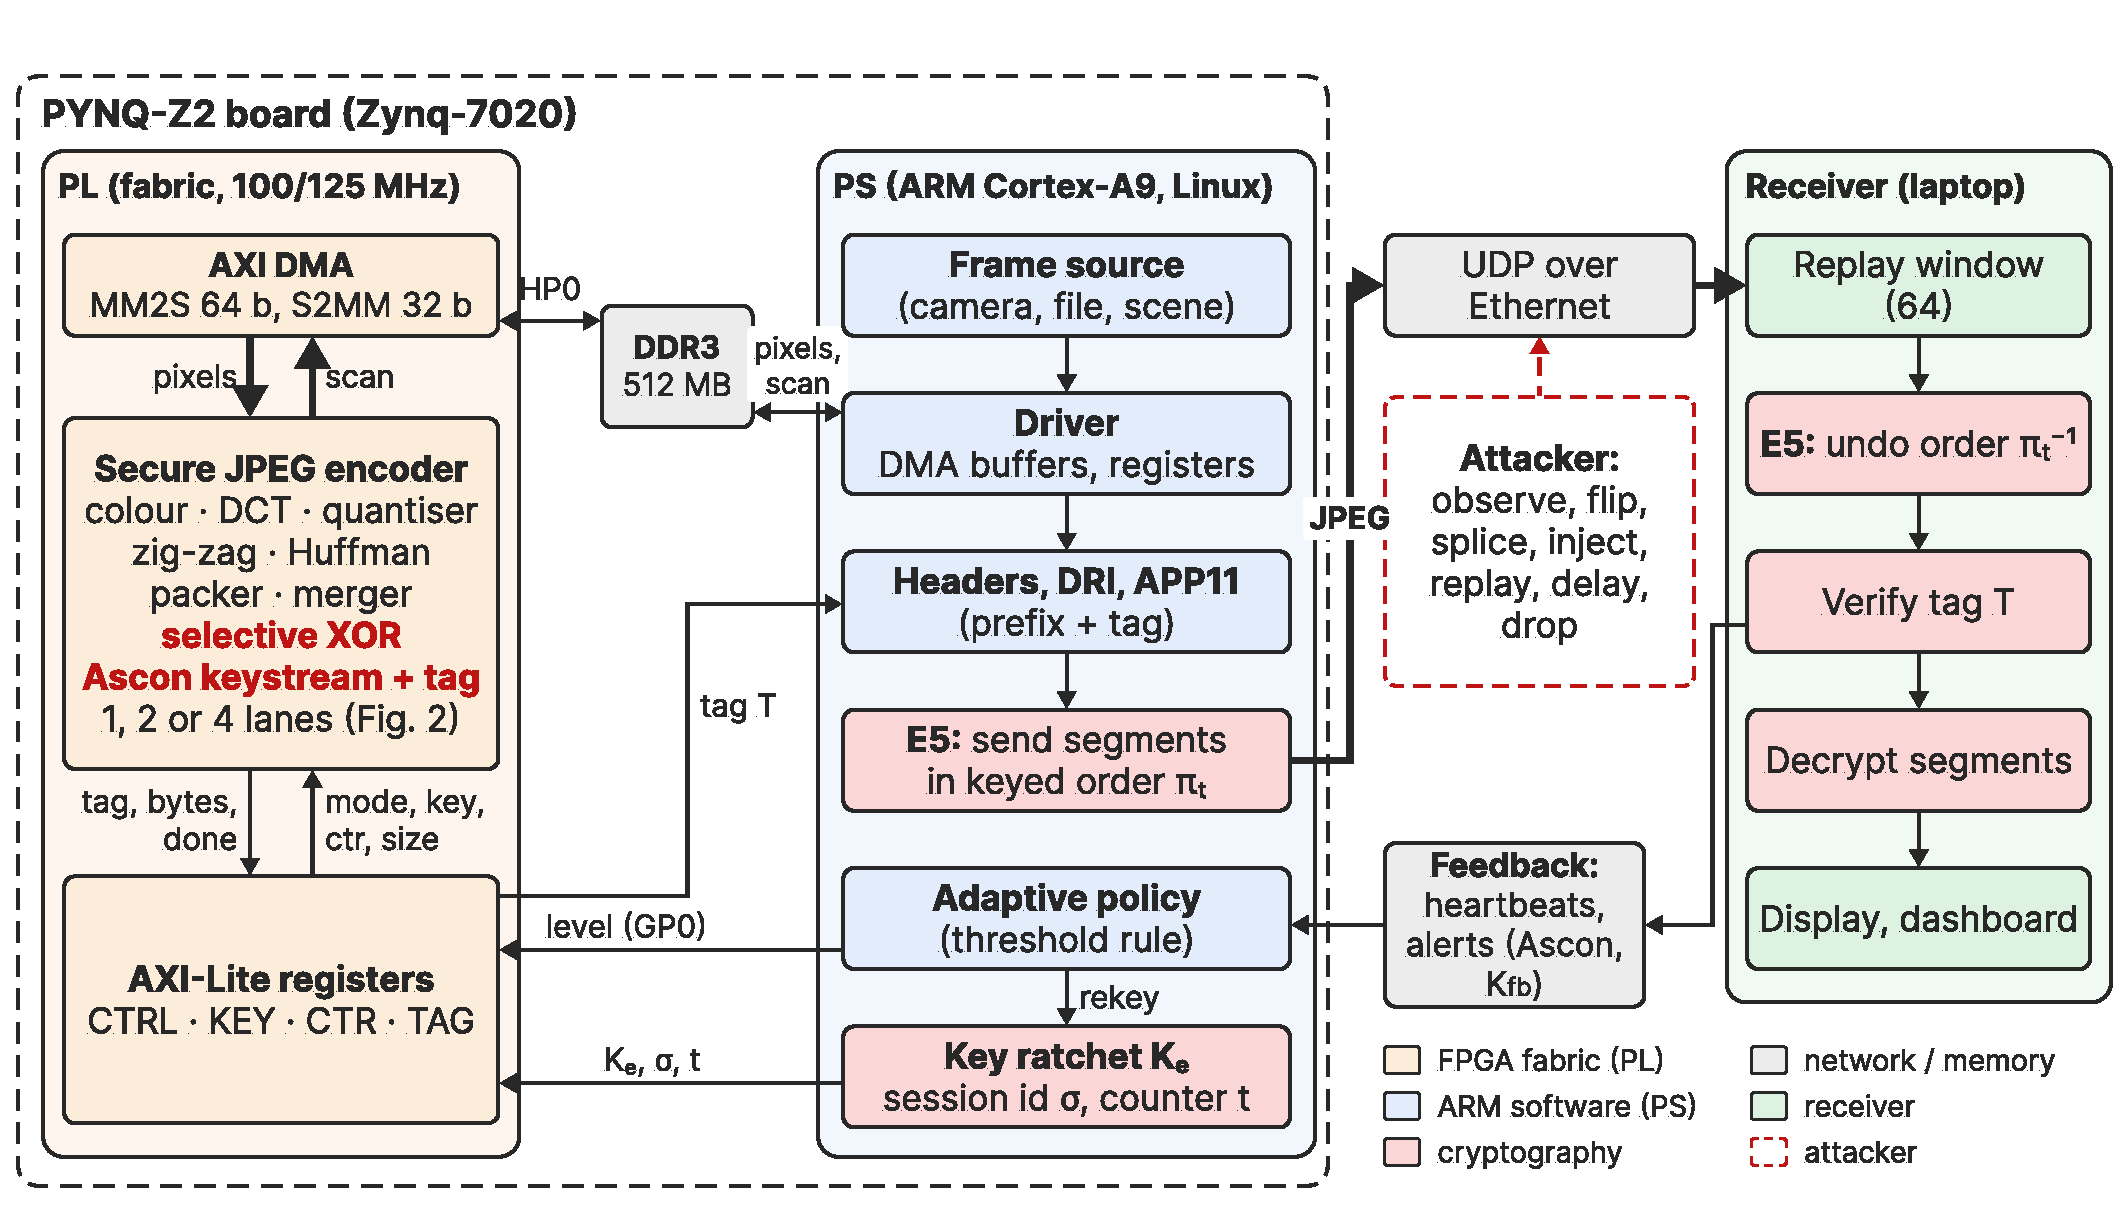
\includegraphics[width=\textwidth]{figures/fig_system.pdf}
\caption{System architecture. The programmable logic (PL) encodes, encrypts and tags every frame; the ARM core (PS) moves pixels and scan through DDR with an AXI DMA, adds the JPEG headers and the tag, sends E5 segments in the keyed order, and runs the key ratchet and the adaptive policy. The receiver undoes the order, verifies the tag, decrypts, and reports back over an authenticated feedback channel. Red: cryptography; dashed: attacker.}
\label{fig:system}
\end{figure*}
Fig.~\ref{fig:system} shows the system. The ARM core places a frame in DDR, writes the per-frame registers and starts the DMA; the fabric codes the pixels into a JPEG scan in which the selected fields are encrypted, computes the frame tag over the metadata and the scan, and writes the scan back. The ARM core wraps it in standard headers and an application segment (APP11) with the tag, reorders the segments under E5, and sends the frame over UDP. All per-byte cryptographic work happens in the fabric.

\subsection{Selective encryption inside the entropy coder}\label{sec:selenc}
\begin{table}[t]
\caption{Protection levels: encrypted fields of every non-zero coefficient (sign: the whole field is inverted; amplitude: its $s{-}1$ low bits) and block positions. Every level carries the tag.}
\label{tab:levels}
\centering\small\setlength{\tabcolsep}{4pt}
\begin{tabular}{lccccc}
\toprule
Level & AC sign & DC sign & AC ampl. & DC ampl. & Positions \\
\midrule
E0 & & & & & \\
E1 & \checkmark & & & & \\
E2 & \checkmark & \checkmark & & & \\
E3 & \checkmark & \checkmark & \checkmark & & \\
E4 & \checkmark & \checkmark & \checkmark & \checkmark & \\
E5 & \checkmark & \checkmark & \checkmark & \checkmark & keyed per frame \\
\bottomrule
\end{tabular}
\end{table}
Table~\ref{tab:levels} lists the six levels; E2 is the default minimum. For a selected symbol with size $s$ and keystream bits $z_0 z_1 \ldots$, the encryption stage computes
\begin{equation}
\amp' = \amp \xor \gamma z_0 (2^s - 1) \xor \alpha \textstyle\sum_{k=1}^{s-1} z_k\, 2^{k-1},
\label{eq:selenc}
\end{equation}
where $\gamma, \alpha \in \{0, 1\}$ say whether the level selects the sign and the amplitude of this coefficient. It consumes $n(s) = \gamma + \alpha (s - 1) \le 11$ keystream bits; decryption is the same XOR.

\begin{lemma}[Format preservation]\label{lem:format}
For every $v \ne 0$ and every keystream, \eqref{eq:selenc} maps $\amp(v)$ to $\amp(v')$ for some $v'$ with $s(v') = s(v)$. Hence the Huffman symbol, the code length and the length of the scan are unchanged, and the encrypted scan is a valid baseline JPEG scan.
\end{lemma}
\begin{IEEEproof}
Let $m = 2^s - 1$. For $v > 0$, $\amp(v) = v$ and $\amp(v) \xor m = m - v = \amp(-v)$ by~\eqref{eq:amp}, and symmetrically for $v < 0$; the sign term is an exact negation. The amplitude term changes only bits $0 \ldots s-2$; bit $s-1$ of $\amp(v)$ is 1 exactly when $v > 0$, and any value of the low bits gives a magnitude in $[2^{s-1}, 2^s - 1]$, i.e.\ size $s$, with the same sign. Neither term touches the run or the Huffman code.
\end{IEEEproof}
The lemma also states what cannot be hidden: the run lengths and size categories stay public at every level E0--E4.

\subsection{Keys, nonces and their uniqueness}\label{sec:nonce}
The master key $K_{\mathrm{m}}$ is the session key that the ARM cores of camera and viewer agree on with a hybrid ML-KEM-768~\cite{fips203} + X25519 exchange authenticated by a pre-shared key. All keys derive from it with one primitive, the Ascon tag used as a pseudorandom function: $\KDF(K, \ell, c) = \MAC_K(N(0, c, 1), \ell)$. The feedback key is $\Kfb = \KDF(K_{\mathrm{m}}, \text{feedback}, 0)$, and the video key follows a one-way ratchet, $K_0 = \KDF(K_{\mathrm{m}}, \text{video}, 0)$, $K_{e+1} = \KDF(K_e, \text{ratchet}, e{+}1)$; each end erases $K_e$ once it has moved on, so a captured key does not decrypt earlier epochs. The 128-bit nonce is
\begin{equation}
N(\sigma, t, b) = \sigma \cat t \cat b, \qquad \sigma = \beta \cat e,
\label{eq:nonce}
\end{equation}
with $\beta$ a 48-bit random base drawn at every boot ($\beta \ne 0$), $e$ the 16-bit epoch, $t$ the 63-bit frame counter and $b$ a purpose bit (0: keystream, 1: tag).

\begin{proposition}[Nonce uniqueness]\label{prop:nonce}
Within one session, no key is used twice with the same nonce, provided the sender never writes the same frame counter twice in an epoch.
\end{proposition}
\begin{IEEEproof}
Under $K_e$ the nonces are $N(\sigma, t, 0)$ for the segment key, $N(\sigma, t, 1)$ for the tag, $N(0, 0, 0)$ for the permutation key and $N(0, c, 1)$ for derivations; $\sigma \ne 0$, $b$ separates the first two, and $t$ is fresh per frame. Under a segment key, a pseudorandom function of $(K_e, \sigma, t)$, the nonces $N(h, t, 0)$ differ in the segment index $h$. A rekey changes both $K_e$ and $\sigma$.
\end{IEEEproof}
With the key exchange every session has a fresh $K_{\mathrm{m}}$. Used directly with the pre-shared key, two boots collide only if they draw the same $\beta$: for $B$ boots this has probability at most $\binom{B}{2} 2^{-48} \approx \BootCollide$ for $B = \BootCount$.

\subsection{Segment keystreams and the frame tag}\label{sec:tag}
Every frame is coded as restart segments (one per MCU row, or one per MCU in E5), each with its own keystream under a per-frame segment key:
\begin{align}
\Kseg &= \MAC_{K_e}\bigl(N(\sigma, t, 0), \text{``lanes''}\bigr), \label{eq:kseg}\\
Z_h &= \Enc_{\Kseg}\bigl(N(h, t, 0), 0^{\ell}\bigr). \label{eq:zs}
\end{align}
Seeking to a segment costs one initialization, which is what lets lanes encrypt independently. The tag authenticates a 26-byte prefix and every byte of the scan, restart markers included:
\begin{equation}
T_t = \MAC_{K_e}\bigl(N(\sigma, t, 1),\ P_t \cat \text{scan}_t\bigr),
\label{eq:tag}
\end{equation}
with $P_t$ = (magic, version, level, $\sigma$, $t$, $W$, $H$). Binding the level matters: an earlier version authenticated only the scan, and a frame could be downgraded from E2 to E1 undetected. The receiver accepts a frame only if~\eqref{eq:tag} verifies and the counter passes a 64-entry replay window as in SRTP~\cite{rfc3711}; a forgery succeeds with probability $2^{-128}$ per attempt.

\subsection{E5: a keyed permutation of macroblocks in hardware form}\label{sec:e5}
\begin{figure}[t]
\centering
\resizebox{\columnwidth}{!}{% E5 in hardware form (docs/INTERFACES.md §8.6): fabric codes MCU segments in raster order and tags them,
% (black bars: restart markers, none after the last segment) the ARM sends them in the keyed order pi_t, the receiver restores raster order before the tag check.
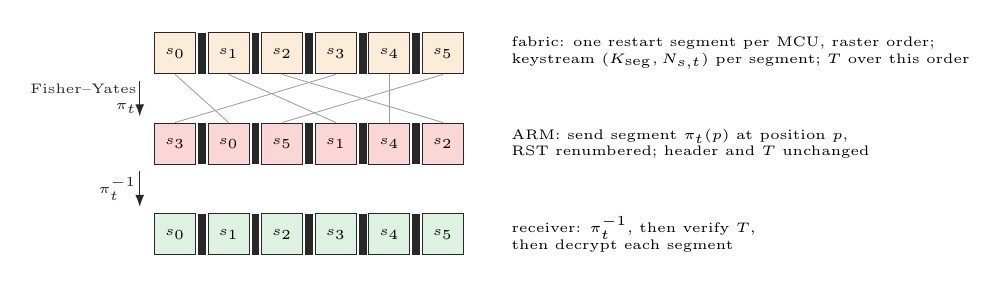
\begin{tikzpicture}[x=1cm, y=1cm,
  seg/.style={draw=inkc, minimum width=5.2mm, minimum height=5.2mm, inner sep=0pt, font=\tiny},
  rst/.style={fill=inkc, minimum width=1.0mm, minimum height=5.2mm, inner sep=0pt},
  st/.style={font=\tiny, align=left, anchor=west}]
\def\segrow#1#2#3{% #1 y, #2 list of labels, #3 fill
  \foreach \l [count=\i from 0] in {#2} {
    \node[seg, fill=#3] at (\i*0.68, #1) {$\l$};
    \ifnum\i<5 \node[rst] at (\i*0.68+0.34, #1) {};\fi
  }}
\segrow{0}{s_0,s_1,s_2,s_3,s_4,s_5}{plfill}
\node[st] at (4.15,0.0) {fabric: one restart segment per MCU, raster order;\\keystream $(K_{\mathrm{seg}}, N_{s,t})$ per segment; $T$ over this order};
\segrow{-1.15}{s_3,s_0,s_5,s_1,s_4,s_2}{cryfill}
\node[st] at (4.15,-1.15) {ARM: send segment $\pi_t(p)$ at position $p$,\\RST renumbered; header and $T$ unchanged};
\segrow{-2.3}{s_0,s_1,s_2,s_3,s_4,s_5}{rxfill}
\node[st] at (4.15,-2.3) {receiver: $\pi_t^{-1}$, then verify $T$,\\then decrypt each segment};
\draw[arr] (-0.45,-0.35) -- node[lbl, left, align=right]{Fisher--Yates\\$\pi_t$} (-0.45,-0.8);
\draw[arr] (-0.45,-1.5) -- node[lbl, left]{$\pi_t^{-1}$} (-0.45,-1.95);
\foreach \a/\b in {0/1,1/3,2/5,3/0,4/4,5/2} {
  \draw[inkc!45, line width=0.3pt] (\a*0.68,-0.27) -- (\b*0.68,-0.88);
}
\end{tikzpicture}
}
\caption{E5 in hardware form. The fabric codes one restart segment per MCU in raster order, each with its own keystream, and tags them in that order; the ARM sends segment $\pi_t(p)$ at wire position $p$; the receiver restores raster order before checking the tag.}
\label{fig:e5}
\end{figure}
Lemma~\ref{lem:format} shows that field encryption cannot hide where the non-zero coefficients are; their count per block alone rebuilds the contours~\cite{hirose2024}. E5 therefore also hides where each macroblock belongs. Permuting macroblocks before entropy coding would need a frame buffer; restart segments allow a cheaper split (Fig.~\ref{fig:e5}). The fabric codes every MCU $h$ as its own segment, encrypted like E4 with $Z_h$, and authenticates the segments in raster order. The ARM splits the scan at the markers and sends segment $\pi_t(p)$ at position $p$, renumbering the markers. The receiver restores raster order with $\pi_t^{-1}$, verifies $T_t$ and only then decrypts. The permutation comes from its own key $K_\pi = \MAC_{K_e}(N(0,0,0), \text{``E5 MCU shuffle''})$ through a Fisher--Yates shuffle on the keystream of $(K_\pi, N(\sigma, t, 0))$, with rejection sampling for uniform indices.

\begin{proposition}[Uniform per-frame permutation]\label{prop:perm}
If the keystream bits are uniform and independent, the shuffle returns each of the $M!$ permutations with probability $1/M!$.
\end{proposition}
\begin{IEEEproof}
At step $i$ a $b_i$-bit draw, $b_i = \lfloor \log_2 i \rfloor + 1$, conditioned on $j \le i$ is uniform on $\{0, \ldots, i\}$; Fisher--Yates with uniform choices produces every permutation exactly once among $\prod_{i=1}^{M-1}(i+1) = M!$ equally likely choice sequences.
\end{IEEEproof}
At 320$\times$240 ($M = \McuQVGA$) the permutation carries $\log_2 M! = \PermBitsQVGA$ bits and costs on average \FyBitsQVGA{} keystream bits. It changes with every frame because $t$ enters the nonce, so the order of one frame says nothing about the next. Because the tag covers the raster-order scan and the receiver derives $\pi_t^{-1}$ from the authenticated $(\sigma, t)$, moving, swapping, dropping or duplicating a segment fails the tag. Each segment adds a two-byte marker, padding and restarted DC prediction, i.e.\ about $M(2 + \tfrac12)$ bytes plus longer DC differences per frame.

\subsection{Authenticated feedback and the adaptive policy}\label{sec:feedback}
The receiver returns an encrypted heartbeat every 0.5\,s and rate-limited alerts (tag failures, replays, malformed or stale frames, loss statistics) under $\Kfb$, with their own counter and replay window. If no valid heartbeat arrives for 3\,s, the sender assumes that the feedback path is attacked: it switches to the highest level and rekeys (dead-man rule). In one-second windows the sender collects the evidence and a threshold policy raises the highest level on any tag failure, replay, feedback attack or flood and holds it for 8\,s; loss counts as jamming only when it is near total, because more encryption cannot help against a degraded network. A contextual bandit~\cite{sutton2018} is the alternative policy: it encrypts fewer bits but reacts later.

% =====================================================================================================
\section{Hardware Architecture}\label{sec:hardware}
\begin{figure*}[t]
\centering
\resizebox{\textwidth}{!}{% Fabric datapath of the contract-v3 lane encoder (rtl/secure_jpeg_lanes_top.v, rtl/encoder_lane.v).
% Bus widths are the RTL port widths; module names are the RTL file names.
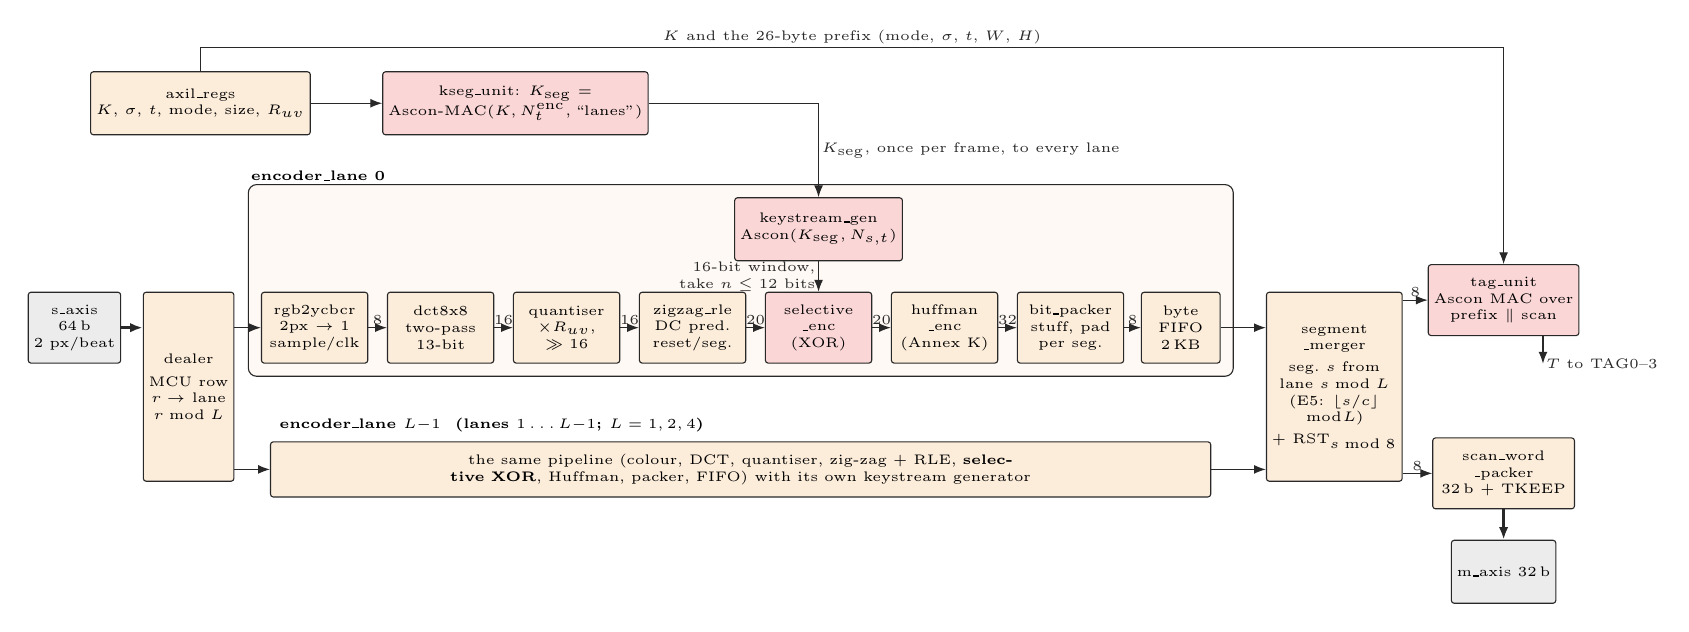
\begin{tikzpicture}[x=1cm, y=1cm, st/.style={pl, minimum height=9mm, minimum width=13.5mm, font=\tiny}]
% ---- input and dealer
\node[blk, fill=netfill, font=\tiny, minimum height=9mm] (in) at (0,0) {s\_axis\\64\,b\\2 px/beat};
\node[pl, font=\tiny, minimum height=24mm, minimum width=11mm, align=center] (deal) at (1.45,-0.75) {dealer\\[2pt]MCU row\\$r\to$ lane\\$r \bmod L$};
\draw[bus] (in) -- (in -| deal.west);
% ---- lane 0 (full) -- y = 0
\node[st] (cc0)  at (3.05,0) {rgb2ycbcr\\2px $\to$ 1\\sample/clk};
\node[st] (dct0) at (4.65,0) {dct8x8\\two-pass\\13-bit};
\node[st] (q0)   at (6.25,0) {quantiser\\$\times R_{uv}$,\\$\gg 16$};
\node[st] (zz0)  at (7.85,0) {zigzag\_rle\\DC pred.\\reset/seg.};
\node[st, fill=cryfill] (se0) at (9.45,0) {selective\\\_enc\\(XOR)};
\node[st] (hu0)  at (11.05,0) {huffman\\\_enc\\(Annex K)};
\node[st] (bp0)  at (12.65,0) {bit\_packer\\stuff, pad\\per seg.};
\node[st, minimum width=10mm] (ff0)  at (14.05,0) {byte\\FIFO\\2\,KB};
\node[cry, font=\tiny, minimum width=19mm, minimum height=8mm] (ks0) at (9.45,1.25) {keystream\_gen\\Ascon$(K_{\mathrm{seg}}, N_{s,t})$};
\draw[arr] (ks0) -- node[lbl, left, align=right]{16-bit window,\\take $n\le 12$ bits} (se0);
\draw[arr] (deal.east |- cc0) -- (cc0);
\draw[arr] (cc0) -- node[lbl, above]{8} (dct0);
\draw[arr] (dct0) -- node[lbl, above]{16} (q0);
\draw[arr] (q0) -- node[lbl, above]{16} (zz0);
\draw[arr] (zz0) -- node[lbl, above]{20} (se0);
\draw[arr] (se0) -- node[lbl, above]{20} (hu0);
\draw[arr] (hu0) -- node[lbl, above]{32} (bp0);
\draw[arr] (bp0) -- node[lbl, above]{8} (ff0);
\begin{scope}[on background layer]
\node[grp, fill=plfill!30, fit=(cc0)(ff0)(ks0), inner sep=1.6mm, label={[font=\tiny\bfseries, anchor=south west, inner sep=1pt]north west:encoder\_lane 0}] (lane0) {};
\end{scope}
% ---- lane L-1 (collapsed) -- y = -1.6
\node[pl, font=\tiny, text width=118mm, minimum height=7mm, align=center] (laneL) at (8.46,-1.8) {the same pipeline (colour, DCT, quantiser, zig-zag + RLE, \textbf{selective XOR}, Huffman, packer, FIFO) with its own keystream generator};
\node[font=\tiny\bfseries, anchor=south west] at (laneL.north west) {encoder\_lane $L{-}1$ \ (lanes $1 \ldots L{-}1$; $L = 1, 2, 4$)};
\draw[arr] (deal.east |- laneL) -- (laneL);
% ---- merger, tag, word packer
\node[pl, font=\tiny, minimum height=24mm, minimum width=13mm, align=center] (mrg) at (16.0,-0.75) {segment\\\_merger\\[2pt]seg.\ $s$ from\\lane $s \bmod L$\\(E5: $\lfloor s/c\rfloor$\\$\bmod L$)\\[2pt]+ RST$_{s \bmod 8}$};
\draw[arr] (ff0.east) -- (ff0.east -| mrg.west);
\draw[arr] (laneL.east) -- (laneL.east -| mrg.west);
\node[cry, font=\tiny, minimum width=18mm, minimum height=9mm] (tag) at (18.15,0.35) {tag\_unit\\Ascon MAC over\\prefix $\|$ scan};
\node[pl, font=\tiny, minimum width=18mm, minimum height=9mm] (wp) at (18.15,-1.85) {scan\_word\\\_packer\\32\,b + TKEEP};
\draw[arr] (mrg.east |- tag) -- node[lbl, above]{8} (tag.west);
\draw[arr] (mrg.east |- wp) -- node[lbl, above]{8} (wp.west);
\node[blk, fill=netfill, font=\tiny, minimum height=8mm] (out) at (18.15,-3.1) {m\_axis 32\,b};
\draw[bus] (wp) -- (out);
% ---- per-frame key, registers
\node[cry, font=\tiny, minimum width=24mm, minimum height=8mm] (kseg) at (5.6,2.85) {kseg\_unit: $K_{\mathrm{seg}}$ =\\Ascon-MAC$(K, N^{\mathrm{enc}}_t, \text{``lanes''})$};
\draw[arr] (kseg.east) -| node[lbl, pos=0.75, right]{$K_{\mathrm{seg}}$, once per frame, to every lane} (ks0.north);
\node[pl, font=\tiny, minimum width=24mm, minimum height=8mm] (regs) at (1.6,2.85) {axil\_regs\\$K$, $\sigma$, $t$, mode, size, $R_{uv}$};
\draw[arr] (regs) -- (kseg);
\draw[arr] (regs.north) -- ++(0,0.3) -| node[lbl, pos=0.25, above]{$K$ and the 26-byte prefix (mode, $\sigma$, $t$, $W$, $H$)} (tag.north);
\draw[arr] (tag.south) ++(0.5,0) -- ++(0,-0.35) node[lbl, right]{$T$ to TAG0--3};
\end{tikzpicture}
}
\caption{Fabric datapath of the lane encoder \texttt{secure\_jpeg\_lanes\_top} (module names are the RTL files; numbers on arrows are bus widths in bits). The dealer sends MCU row $r$ to lane $r \bmod L$; each lane converts, transforms, quantizes and entropy-codes its restart segments with its own keystream; the merger restores raster order and inserts restart markers; the tag unit authenticates the prefix and the merged scan. The single-pipeline encoder is one lane without dealer and merger.}
\label{fig:pl}
\end{figure*}
\subsection{Datapath}\label{sec:datapath}
Fig.~\ref{fig:pl} shows the encoder. All stages are joined by valid/ready handshakes and tolerate back-pressure from the DMA, which the testbenches check with random stalls. The colour converter takes two pixels per clock into block-RAM line buffers, the DCT is two passes of an eight-tap multiply-accumulate, the quantizer multiplies by a reciprocal table in one DSP slice, and the zig-zag stage emits one symbol per clock and resets its DC predictors at every segment, ahead of encryption, Huffman coding and byte packing. The merger copies the segments of all lanes in raster order and writes the restart markers, and the tag unit absorbs the prefix and every merged byte into an Ascon core.

\subsection{Circuit of the encryption stage}\label{sec:circuit}
\begin{figure}[t]
\centering
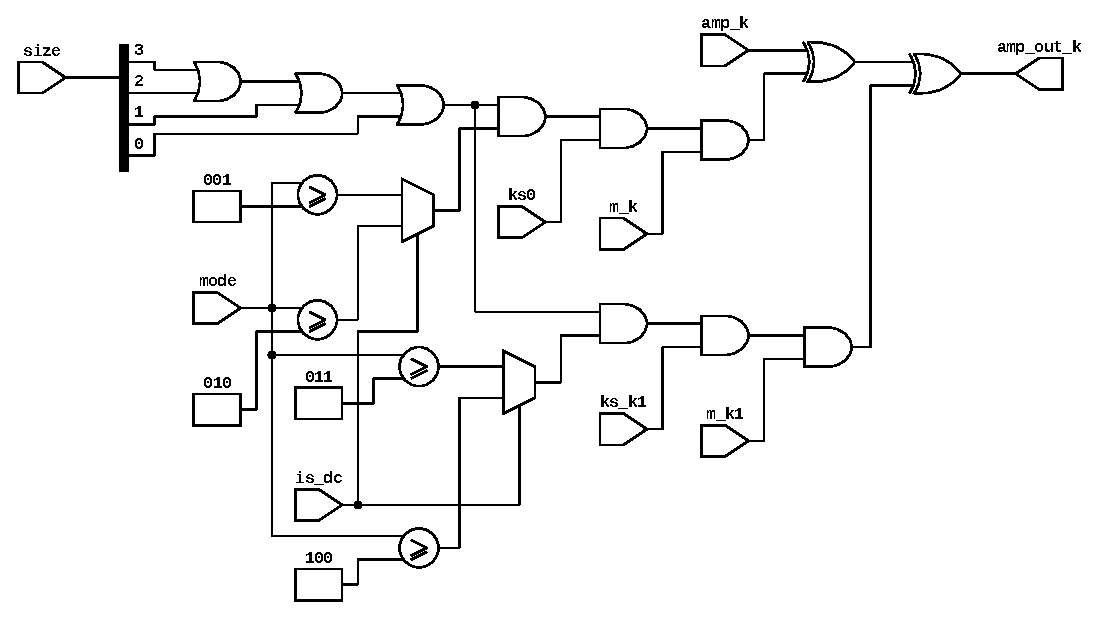
\includegraphics[width=\columnwidth]{figures/fig_selective_enc_bitslice.pdf}
\caption{Gate-level circuit of bit slice $k$ of \texttt{selective\_enc.v}, generated from the RTL by Yosys and netlistsvg: comparators on the mode and multiplexers selected by is\_dc form the sign and amplitude enables; two XORs implement~\eqref{eq:slice}. $m_k = [k < s]$; ks0 and ks\_k1 are keystream bits 0 and $k{+}1$. A test simulates the slice exhaustively against the golden model.}
\label{fig:circuit}
\end{figure}
Fig.~\ref{fig:circuit} is one bit slice of the stage. The control part decodes $\gamma = [s \ne 0] \wedge (\text{is\_dc} \mathbin{?} \text{mode} \ge 2 : \text{mode} \ge 1)$ and $\alpha = [s \ne 0] \wedge (\text{is\_dc} \mathbin{?} \text{mode} \ge 4 : \text{mode} \ge 3)$; mode 5 selects the fields of mode 4 because all comparisons are $\ge$. The data part is eleven identical slices,
\begin{equation}
\amp'_k = \amp_k \xor (\gamma z_0 \wedge m_k) \xor (\alpha z_{k+1} \wedge m_{k+1}), \quad m = 2^s - 1,
\label{eq:slice}
\end{equation}
one XOR deep after the masks, which are computed one register earlier. The stage accepts a symbol when its output is free and at least $n$ keystream bits are available.

\textit{Keystream window.} \texttt{keystream\_gen} holds two 128-bit blocks and a pointer to the next unused bit and presents a 16-bit window; taking $n$ bits advances the pointer, and a new block is requested whenever fewer than two are held or in flight.

\begin{proposition}[The cipher never stalls the encoder]\label{prop:supply}
Once the first keystream block of a segment is available, the encryption stage never waits for keystream bits.
\end{proposition}
\begin{IEEEproof}
The stage accepts at most one symbol per clock and takes at most 11 bits per symbol. The core produces 128 bits per data block in nine cycles (one to absorb, eight rounds), more than 14 bits per cycle, and keeps up to 256 bits buffered, more than the 16 that the window exposes. Supply exceeds the worst-case demand, so the window, once filled, never drops below what a symbol needs.
\end{IEEEproof}
The first block of a segment costs an initialization and one data block, 21 cycles, which overlaps with the previous segment; RTL simulation confirms that the cycle counts of E0--E4 differ by at most \MaxExtraCycles{} cycles per frame.

\textit{Ascon core.} \texttt{ascon\_aead128\_core} computes one round per clock: a 320-bit state register, a 4-bit round counter whose complement and value form the round constant, and the combinational round. One bit slice of the S-box layer has eleven XOR, five AND and six NOT gates, so the layer has $64 \times 22 = 1408$ gates; the linear layer adds $2 \times 320$ two-input XORs, and its rotations are wiring. The design instantiates one core per lane for keystreams, one for the segment key and one for the tag.

\subsection{Parallel lanes}\label{sec:lanes}
One pipeline consumes one sample per clock, i.e.\ at least 1.5 cycles per pixel. Restart segments are independent (DC predictors reset, byte alignment, own keystream), so $L$ pipelines can code segments simultaneously: the dealer sends MCU row $r$ to lane $r \bmod L$ and the merger reads segment $h$ from its lane (under E5 from lane $\lfloor h/c \rfloor \bmod L$ with $c = W/16$, tracked by counters). With a 64-bit input carrying two pixels per clock,
\begin{equation}
c_L \ge \max\Bigl(\frac{1.5}{L}, \frac{1}{2}\Bigr), \qquad \Theta_L = \frac{f_{\mathrm{clk}}}{c_L},
\label{eq:lanes}
\end{equation}
i.e.\ at most \BoundOneMpix, \BoundTwoMpix{} and \BoundFourMpix\,Mpixel/s at 100\,MHz for $L = 1, 2, 4$. The bytes do not depend on $L$. A lane encoder can also be built for a camera's YUYV (4:2:2) input: four pixels per beat, no colour multipliers, a bound of $\max(1.5/L, 1/4)$ and half the bytes read from DDR.

\subsection{System and timing closure}\label{sec:zynq}
A script builds the PYNQ-Z2 system in Vivado: the Zynq processing system, an AXI DMA on the 64-bit high-performance port and the encoder as a module reference, all on one clock (100\,MHz, or 125\,MHz for four lanes). The register map holds the key, session identifier, counter, size, mode, tag, output length and three cycle counters (start to done, waiting for pixels, waiting for the output DMA), so the board reports the fabric's own time. Timing closure needed four changes, each accepted only when every RTL test still matched the model bit for bit: a five-stage pipeline for the DCT row sums (the first implementation reached only about 47\,MHz after routing), registered pixel conversion in the complete system, a zig-zag stage split into two handshaked stages, and two-entry register slices that cut the ready chain from the packer back to the keystream pointer.

% =====================================================================================================
\section{Hardware Results}\label{sec:hwresults}
\subsection{Verification}\label{sec:verification}
A Python golden model is the referee for every RTL stage; its Ascon passes all 1089 official known-answer tests, as does the RTL core. Every RTL module has a cocotb testbench with random idle cycles and back-pressure that reports the first mismatch, and the complete encoders are byte-exact with the model for every level and for one, two and four lanes, in Icarus Verilog and in Vivado's simulator. Every defect found received a regression test and a root cause.

\subsection{Cycles, area and timing}
In RTL simulation the cycle counts of E0--E4 differ by at most \MaxExtraCycles{} cycles per frame, which is handshake noise: as Proposition~\ref{prop:supply} predicts, encryption costs no cycles. Above the floor of 1.5 cycles per pixel the only cost of a single pipeline is filling the first MCU row, $c_1(r) = 1.5 + \FillA/r$ for $r$ MCU rows (\CppVGA{} at 640$\times$480). One, two and four lanes reach \RtlOneLaneMpix, \RtlTwoLanesMpix{} and \RtlFourLanesMpix\,Mpixel/s at 100\,MHz, against the bounds \BoundOneMpix, \BoundTwoMpix{} and \BoundFourMpix{} of~\eqref{eq:lanes}; E5, with one restart per MCU, costs a few per cent.

% generated by paper/make_assets.py from paper/data -- do not edit
\begin{table}[t]
\caption{Resources on the xc7z020 (53\,200 LUT, 106\,400 FF, 140 BRAM36, 220 DSP). Source: Vivado post-route, out of context, 100\,MHz with I/O delays of 20\,\% of the period, WNS +0.630\,ns.}
\label{tab:resources}
\centering\small
\resizebox{\columnwidth}{!}{%
\begin{tabular}{lrrrr}
\toprule
Block & LUT & FF & BRAM36 & DSP \\
\midrule
Encoder (all) & 4785 (9.0\%) & 3051 (2.9\%) & 25.5 (18.2\%) & 23 (10.4\%) \\
\quad colour conversion + line buffers & 459 & 220 & 25 & 0 \\
\quad DCT and quantizer & 806 & 69 & 0 & 22 \\
\quad zig-zag, Huffman, packing & 717 & 323 & 0 & 0 \\
\quad keystream generator (Ascon) & 949 & 851 & 0 & 0 \\
\quad tag unit (Ascon) & 1358 & 1072 & 0 & 0 \\
\quad selective encryption & 82 & 24 & 0 & 0 \\
\quad AXI-Lite registers & 392 & 451 & 0 & 0 \\
\bottomrule
\end{tabular}}
\end{table}

After place and route the single pipeline meets \TopMhz\,MHz on the xc7z020 (WNS $+$\TopWns\,ns, out of context) with \TopLuts{} LUTs (\TopLutPct\,\% of the device, Table~\ref{tab:resources}); the two Ascon instances take \CryptoLutShare\,\% of them and the selective-encryption stage is tiny. With switching activity from simulating a real frame it draws about \SaifTopMw\,mW. Two lanes take \TwoLanesLuts{} LUTs and four lanes \FourLanesLuts{}; E5 adds no BRAM or DSP. Out of context one, two and four lanes also meet 150\,MHz (WNS \TopWnsAtOneFifty, \LanesTwoWnsAtOneFifty{} and \LanesFourWnsAtOneFifty\,ns). The complete PYNQ-Z2 systems close timing: one and two lanes at \OverlayMhz\,MHz, four lanes at \OverlayLanesFourMhz\,MHz with \OverlayLanesFourLuts{} LUTs (\OverlayLanesFourLutPct\,\% of the device).

% generated by paper/make_assets.py from paper/data -- do not edit
\begin{table}[t]
\caption{Comparison with published FPGA designs. Their numbers are as reported by each source; ours are
post-route (Table~\ref{tab:resources}) with throughput from the RTL cycle count. Mpx/s: million pixels per second.}
\label{tab:compare}
\centering\small
\resizebox{\columnwidth}{!}{%
\begin{tabular}{llrrrrrl}
\toprule
Design & Device & LUT & BRAM & DSP & MHz & Mpx/s & Crypto \\
\midrule
Ours: encoder & Zynq-7020 & 5{,}039 & 24.5 & 23 & 100 & 61 & sel.\ AEAD \\
Ours: one Ascon & Zynq-7020 & 860--969 & 0 & 0 & 100 & -- & AEAD core \\
logiJPGE~\cite{logijpge} & Zynq-7020 & 3{,}240 & 16 & 30 & 150 & 150 & none \\
CAST JPEG-E-S~\cite{castjpeg} & Artix-7 & 3{,}069 & 2 & 16 & 166 & -- & none \\
Khairallah~\cite{khairallah2023} & Artix-7 & 1{,}031 & 0 & 0 & 200 & -- & MAC \\
Kurian~\cite{kurian2025} & Artix-7 & 5{,}335 & 32 & 0 & 100 & -- & AEAD \\
\bottomrule
\end{tabular}}
\end{table}

\textit{Comparison.} Table~\ref{tab:compare} sets the design against published FPGA work. Each Ascon core (\AsconLutMin--\AsconLutMax{} LUTs) is as small as the round-per-cycle Ascon cores of~\cite{khairallah2023}; the commercial encoders~\cite{logijpge,castjpeg} use less block RAM and no cryptography. Per thousand LUTs, one and four lanes give \HeTopPerKlut{} and \HeFourPerKlut\,Mpixel/s against \HeKishorePerKlut{} for the scrambling encoder of Kishore et al.~\cite{kishore2015}.

\subsection{Board evaluation}\label{sec:board}
% generated by paper/make_assets.py from paper/data -- do not edit
\begin{table*}[t]
\caption{On the PYNQ-Z2 (24 Oct 2026): the final board images, each at the clock it was built for, and the same
function on the board's ARM Cortex-A9. Bit-exact: every frame of every level compared byte for byte (scan and tag)
with the golden model running on the board (58 frames in all). Fabric: START to DONE from
the encoder's CYCLES register for one 640$\times$480 frame (Mpixel/s in brackets); wait: share of those cycles in
which the encoder could take a pixel but the DMA had none, mostly because the Python driver starts the DMA after the encoder. Frame: a complete authenticated JPEG with headers (and
for E5 the segment order) on the ARM, the pixels already in the DMA buffer as a camera would leave them, median of
50 frames (frames/s in brackets). ARM rows: median of 30 frames; ``file'' encrypts the whole JPEG, so it does not
play without the key.}
\label{tab:board}
\centering\small\setlength{\tabcolsep}{4pt}
\resizebox{\textwidth}{!}{%
\begin{tabular}{lrlrrrr}
\toprule
Encoder & MHz & Bit-exact & Fabric, ms & Wait (\%) & E2 frame, ms & E5 frame, ms \\
\midrule
4 lanes & 125 & E0--E5 & 1.97 (156) & 31 & 5.9 (169) & 8.4 (119) \\
2 lanes & 100 & E0--E5 & 3.06 (100) & 21 & 7.0 (144) & 9.8 (102) \\
1 lane & 100 & E0--E4 & 5.34 (58) & 12 & 9.2 (108) & -- \\
\midrule
ARM, ours in C, 1 core & -- & E0--E5 & -- & -- & 114.2 (8.8) & 133.0 (7.5) \\
ARM, ours in C, 2 cores & -- & E0--E5 & -- & -- & 61.6 (16.2) & 74.8 (13.4) \\
ARM, libjpeg-turbo, no security & -- & -- & -- & -- & 28.8 (34.8) & -- \\
ARM, libjpeg-turbo + Ascon (file) & -- & -- & -- & -- & 31.7 (31.5) & -- \\
ARM, libjpeg-turbo + AES-GCM (file) & -- & -- & -- & -- & 31.9 (31.3) & -- \\
\bottomrule
\end{tabular}}
\end{table*}

\begin{figure}[t]
\centering
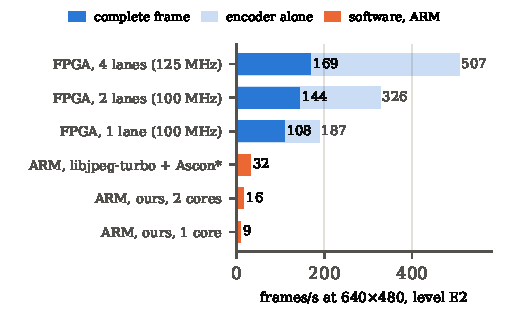
\includegraphics[width=\columnwidth]{figures/fig_board_fps.pdf}
\caption{Measured on the PYNQ-Z2: authenticated 640$\times$480 frames per second (E2) of the three board images, each at the clock it was built for, and of software on the board's two Cortex-A9 cores. Light: the encoder alone, START to DONE from its cycle counter. *Encrypts the whole file, so it does not play without the key.}
\label{fig:boardfps}
\end{figure}
The board evaluation has four parts, all scripted and rehearsed against an emulation of the bitstream: (A1) a bit-exact gate that encodes frames in every level on the fabric and compares every byte and tag with the golden model running on the board; (A2) the fabric's own time from its cycle counters and the time of a complete frame; (A3) the same function on the board's processing system; and (A4) energy per frame. Table~\ref{tab:board} gives the results.

\textit{Correctness.} All \BdImages{} board images, one, two and four lanes, are bit-exact with the golden model in every level they implement (\BdFramesTotal{} frames, every scan byte and tag). The board thus confirms Lemma~\ref{lem:format} and the lane, E5 and tag logic on silicon.

\textit{Speed.} The images count the clocks from start to done and, among them, the clocks in which the encoder could take a pixel but the DMA had none. Without those waits the counts equal the RTL simulation to within \BdBusyVsRtlMaxPct\,\% for every image: four lanes at \BdFourMhz\,MHz encode a 640$\times$480 frame in \BdFourBusyMs\,ms (\BdFourBusyMpix\,Mpixel/s), and the encoding clocks of E0--E4 differ by at most \BdFourBusySpreadClk{} per frame, so encryption costs no time on silicon either. The waits are almost the same for every image, \BdWaitMsMin--\BdWaitMsMax\,ms per frame, because our Python driver writes START before it starts the pixel DMA. With the pixels already in the DMA buffer, as a camera writing there would leave them, a complete authenticated frame takes \BdFourZcMs\,ms (\BdFourZcFps{} frames/s, Fig.~\ref{fig:boardfps}); the DMA transfers and the headers on the ARM, not the encoder, set this rate, and E5 adds \BdFourEfiveExtraMs\,ms for reordering the segments.

\textit{The ARM baseline.} Our encoder in C, gated bit-exact against the model, encodes a 640$\times$480 E2 frame in \BdArmOursTwoMs\,ms on both Cortex-A9 cores (\BdArmOursTwoFps{} frames/s); libjpeg-turbo takes \BdArmTurboMs\,ms alone and \BdArmTurboAsconMs\,ms with whole-file Ascon-AEAD128, whose output does not play without the key. The FPGA's complete frame is \BdSpeedupFrame{} times faster than our encoder on both cores and \BdSpeedupTurboAscon{} times faster than libjpeg-turbo with Ascon.

\textit{Energy.} Without an inline meter, the energy per frame combines the measured frame rate with Vivado's post-route power of the complete four-lane system (\BdPowerEstW\,W, processing system included): \BdEnergyEtwoMj\,mJ per E2 frame and \BdEnergyEfiveMj\,mJ per E5 frame. This is an estimate, not a measurement.

% =====================================================================================================
\section{Security Evaluation}\label{sec:security}
\textit{Setup.} We measure what a keyless observer can reconstruct. For every frame we take the better of two pictures: the protected stream decoded as is, and a \emph{replacement attack} that substitutes fixed guesses for the encrypted values and re-encodes a valid JPEG. Leakage is the edge correlation $\rho_E$, the Pearson correlation between the Sobel gradient magnitudes of this picture and of the original ($\rho_E = 0$: no outline); it is insensitive to brightness and contrast, which a learned attacker recovers from global statistics. We also report SSIM~\cite{ssim}. Sources are a synthetic scene, \NumClips{} private clips that we analyse but do not reproduce, \NumOpenClips{} openly licensed films of the Blender Foundation and the 24 Kodak images, at 320$\times$240. The protected streams of \AllDecode{} six levels decode without error in \Decoders, as Lemma~\ref{lem:format} requires.

\subsection{Outline leakage}\label{sec:leakage}
\begin{figure*}[t]
\centering
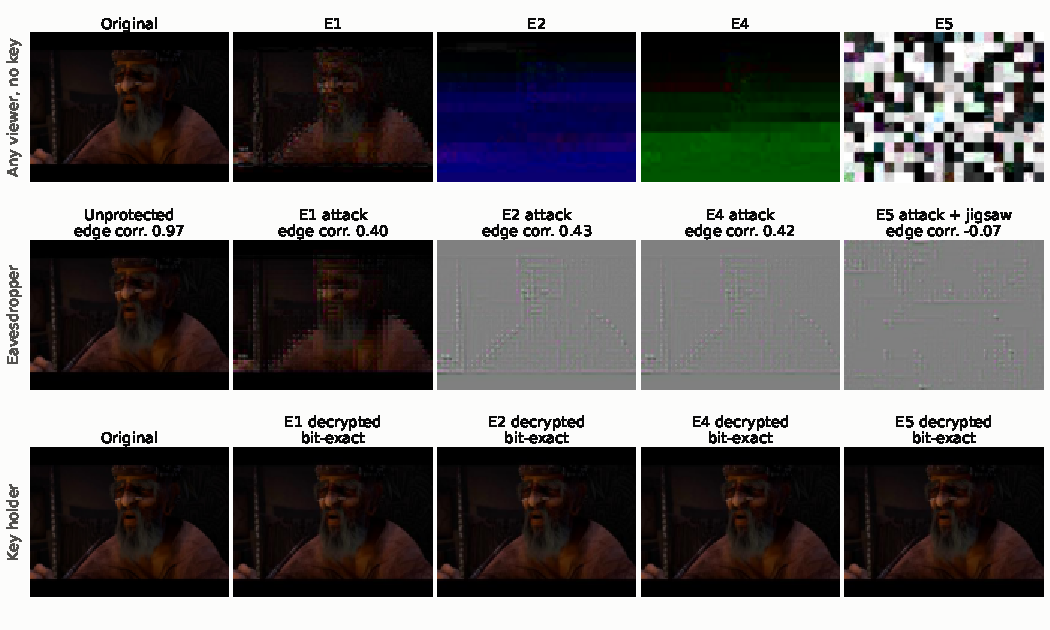
\includegraphics[width=0.62\textwidth]{figures/fig_visual_grid.pdf}
\caption{One frame of the Sintel trailer (\copyright{} Blender Foundation, CC~BY~3.0) per protection level. Top: what any viewer shows without the key. Middle: the eavesdropper's best reconstruction (for E5 after the jigsaw solver) with its edge correlation. Bottom: the key holder's output, bit-exact.}
\label{fig:grid}
\end{figure*}
% generated by paper/make_assets.py from paper/data -- do not edit
\begin{table}[t]
\caption{Outline leakage: edge correlation between the original and the eavesdropper's best keyless reconstruction (decode or replacement attack; 0 = no outline), up to 20 frames per source; frames without edges are skipped. The first row is the fraction of payload bits encrypted.}
\label{tab:leakage}
\centering\small\setlength{\tabcolsep}{4pt}
\resizebox{\columnwidth}{!}{%
\begin{tabular}{lrrrrrr}
\toprule
Source & E0 & E1 & E2 & E3 & E4 & E5 \\
\midrule
Enc.\ share & 0.00 & 0.11 & 0.13 & 0.26 & 0.30 & 0.31 \\
\midrule
Synthetic & 1.00 & 0.38 & 0.36 & 0.37 & 0.37 & 0.00 \\
Trailer A & 0.99 & 0.47 & 0.34 & 0.34 & 0.33 & 0.01 \\
Trailer B & 0.99 & 0.58 & 0.27 & 0.31 & 0.30 & 0.02 \\
Talk A & 0.99 & 0.50 & 0.44 & 0.44 & 0.44 & -0.00 \\
Talk B & 0.99 & 0.49 & 0.38 & 0.44 & 0.43 & 0.01 \\
Sintel & 0.99 & 0.35 & 0.25 & 0.26 & 0.27 & -0.00 \\
Tears of Steel & 0.99 & 0.47 & 0.34 & 0.35 & 0.43 & -0.01 \\
Kodak & 0.99 & 0.39 & 0.32 & 0.33 & 0.30 & 0.00 \\
\bottomrule
\end{tabular}}
\end{table}

Under E1--E4 the eavesdropper sees the outline of the scene (edge correlation \LeakEOneFourMin--\LeakEOneFourMax, Table~\ref{tab:leakage}, Fig.~\ref{fig:grid}), and encrypting amplitudes in addition to signs does not reduce it, because positions and size categories stay public. E5 removes the outline (\LeakEFiveMin{} to \LeakEFiveMax) for \CostEfive\,\% encrypted bits, against \CostEfour\,\% for E4, at \RiOverheadOneMin--\RiOverheadOneMax\,\% more bytes for the restart markers. Longer restart intervals would cost less, but a beam-search solver that chains segments by border continuity links many of them to their true successor at 32 MCUs per segment, so we keep one MCU per segment.

\subsection{Published schemes under the same attacks}\label{sec:bench}
\begin{figure}[t]
\centering
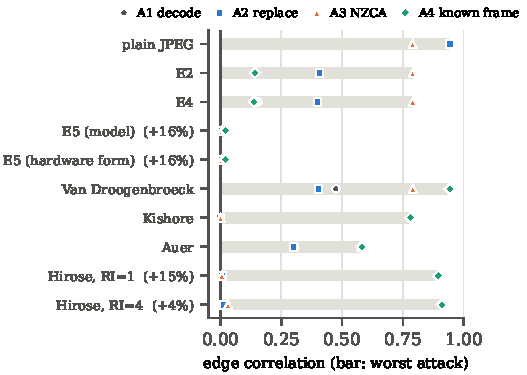
\includegraphics[width=\columnwidth]{figures/fig_bench.pdf}
\caption{SVE-Bench: edge correlation of every scheme under each attack, pooled over \BenchSources{} sources; the bar ends at the worst attack. Byte cost over plain JPEG in brackets when above 2\,\%.}
\label{fig:bench}
\end{figure}
Leakage numbers from different papers are not comparable, so we re-implemented four format-compliant schemes~\cite{vandroogenbroeck2002,kishore2015,auer2013,hirose2024} with our keystream and scored them and ours under the same four attacks on \BenchFrames{} frames of \BenchSources{} sources (Fig.~\ref{fig:bench}): A1 decoding, A2 replacement, A3 non-zero counting (a picture built from the number of non-zero coefficients per block~\cite{hirose2024}), and A4, a known-plaintext attacker that recovers the permutation and keystream bits of one frame and applies them to the next. At its strongest attack every published scheme leaks \BenchPubMin--\BenchPubMax. Fixed key material falls to A4, among them Hirose et al.\ with a restart marker after every block (\BenchHiroseOneCross), although it costs about as many bytes as E5. E1--E4 sit at the non-zero-counting ceiling of plain JPEG (\BenchPlainNzca). E5, keyed anew per frame (Proposition~\ref{prop:perm}), stays at or below \BenchEfiveMax{} in both its model and hardware form; the mechanism is the one of Hirose et al., the difference is the per-frame key.

\subsection{Stronger attackers}
\textit{Puzzle solvers and chosen plaintext.} A greedy solver in the style of~\cite{pomeranz2011} and a minimum-spanning-tree solver with gradient compatibility~\cite{gallagher2012}, both of which reassemble unencrypted shuffled tiles well, place at most \JigsawNeighboursMax{} and \MstNbMax\,\% of E5 neighbours correctly, i.e.\ chance: the signs and amplitudes are also encrypted, so tile borders no longer match. A chosen-plaintext attacker who films a pattern that reveals one frame's permutation~\cite{li2025shuffle} places \CpaPlacedEfive\,\% of the next frame's tiles, because the permutation comes from the frame nonce.

\textit{Sign recovery.} The linear program of Lin et al.~\cite{lin2024} recovers \SrLinSignsMin--\SrLinSignsMax\,\% of the signs in its own setting, where only a few signs per block are unknown, but \SrEoneSigns\,\% of E1's and \SrEtwoSigns\,\% of E2's (chance 50\,\%) on \SrFrames{} frames of \SrSources{} source sets.

\textit{Learned attackers.} A U-Net~\cite{unet} trained on \LearnBigTrain{} frames and tested on unseen sources breaks E1 (edge correlation \LearnEoneEdge, SSIM \LearnEoneSsim; replacement attack \ReplEoneEdge), adds little to the outline under E2 and E4 (\LearnEtwoFourEdge{} against \ReplEtwoFourEdge), and under E5 learns only brightness and colour: SSIM \LearnEfiveSsimBig{} against \CtrlTrueSsim{} for an oracle that recolours the median training frame with each test frame's true statistics, and edge correlation \LearnEfiveEdgeBig{} against \CtrlTrueEdge. A variant trained on public films with an adversarial loss from a PatchGAN discriminator~\cite{isola2017} recovers nothing more under E5.

\textit{Recognition.} An off-the-shelf person detector, Faster R-CNN~\cite{ren2015}, finds \RecPlainMin--\RecPlainMax\,\% of the \RecPersons{} persons in unprotected frames, \RecEonePooled\,\% in the eavesdropper's pictures under E1 (pooled), at most \RecEtwoFourMax\,\% on any source under E2 and E4, and none under E5.

\subsection{What no level hides}\label{sec:sizes}
Encryption hides content, not length. Frame sizes reveal motion at every level alike, and identify a known video as for encrypted streaming~\cite{schuster2017}: from ten frame sizes an attacker picks the right one of \FpVideos{} videos \FpEtwoTen\,\% of the time under E2 and \FpEfiveTen\,\% under E5 (chance \FpChance\,\%). Only constant-size frames reach chance, at up to $+$\PadFilmMax\,\% bytes on edited clips but $+$\PadFixed\,\% for a fixed camera, the favourable case of a home camera. The link pads every frame to the largest size so far as an option, in a comment segment that decoders skip and the tag need not cover. Standard image-encryption metrics~\cite{massoudi2008} assume a cipher that turns the image into noise; key sensitivity holds (a one-bit key change alters \StdNpcrEfiveMin--\StdNpcrEfiveMax\,\% of E5's pixels), and in practice such a frame fails its tag.

% =====================================================================================================
\section{Protocol and Defence Evaluation}\label{sec:protocol}
% generated by paper/make_assets.py from paper/data -- do not edit
\begin{table}[t]
\caption{Reaction to each active attack (full suite, threshold policy, 3 runs; mean\,$\pm$\,s.d. in seconds). ``First rejection'' is when the receiver first discards a frame; ``mitigated'' is when the sender has raised protection or rekeyed.}
\label{tab:attacks}
\centering\small\setlength{\tabcolsep}{4pt}
\resizebox{\columnwidth}{!}{%
\begin{tabular}{lccc}
\toprule
Attack & Mitigated & First rejection & Mitigated after \\
\midrule
bit flips in the scan & 3/3 & 0.09\,$\pm$\,0.03 & 0.41\,$\pm$\,0.02 \\
mode downgrade in header & 3/3 & 0.06\,$\pm$\,0.02 & 0.44\,$\pm$\,0.02 \\
splice of two frames & 3/3 & 0.13\,$\pm$\,0.00 & 0.46\,$\pm$\,0.01 \\
forged frame injection & 3/3 & 0.14\,$\pm$\,0.06 & 0.44\,$\pm$\,0.03 \\
frame replay & 3/3 & 0.07\,$\pm$\,0.05 & 0.46\,$\pm$\,0.03 \\
frame delay & 3/3 & 4.13\,$\pm$\,0.04 & 1.46\,$\pm$\,0.03 \\
frame dropping & 3/3 & -- & 1.46\,$\pm$\,0.03 \\
junk flood & 3/3 & -- & 0.49\,$\pm$\,0.04 \\
feedback dropping & 3/3 & -- & 3.47\,$\pm$\,0.05 \\
forged feedback & 3/3 & -- & 0.46\,$\pm$\,0.04 \\
feedback replay & 3/3 & -- & 0.44\,$\pm$\,0.01 \\
\bottomrule
\end{tabular}}
\end{table}

\textit{Setup.} Sender, network channel with the attacker, and receiver run as separate processes over UDP, so the evaluation exercises the real wire format, fragmentation and timing (320$\times$240, 10 frames/s, datagrams of at most 1400 bytes). The full scenario applies \NumAttacks{} attacks for six seconds each, 25\,s apart: bit flips in the scan, a mode downgrade, splicing, injection of a forged frame, replay, delay, dropping, a junk flood, and dropping, forging and replaying feedback.

\textit{Results.} Over \SuiteRuns{} runs every attack was mitigated, on average \TtmMean{}\,$\pm$\,\TtmSd{}\,s after it began, with \SuiteFalse{} false alarms in calm windows (Table~\ref{tab:attacks}). With the PYNQ-Z2 as the sender, the same suite was again mitigated in full (\BdSuiteMit, column ``Board'') without a false alarm in \BdSuiteFalse{} calm windows, each attack within about one decision window. The evidence, not the harm, sets the reaction time: a bit flip fails the tag at the first frame, held-back frames produce no rejection while they are held, and silenced feedback blinds the sender until the dead-man rule fires after \FbDropTtm\,s. Integrity attacks are therefore caught at once; attacks by absence only by a timeout, whose length trades against false alarms on a slow network.

\textit{Benign impairments.} A second scenario applies only network problems: packet loss rising to 6\,\%, delay with jitter, and reordering. Over \BenignRuns{} runs the defence raised no false alarm (\BenignFalse{} windows), and none on the board (\BdBenignFalse{}). At \CaseSixPct\,\% packet loss the receiver lost \CaseSixFrameLoss\,\% of the frames, because a frame is lost when any of its fragments is; loss between 5 and 90\,\% is reported as a degraded network, not an attack, so jamming that lets more than a tenth of the frames through is indistinguishable from a bad network.

\textit{Fault injection inside the camera.} A variant of the two-lane board image places a fault injector between the encoder and the receive DMA, after the tag is computed, which flips one non-marker bit of the scan on a trigger. It stands for a fault or an implant anywhere on the path from the DMA through memory, the ARM and the network card. All \BdTamperShots{} triggered flips were detected and no other frame was rejected; \BdTamperOneFrame{} triggers cost exactly one frame and \BdTamperTwoFrames{} cost two, most likely because the trigger input is not debounced.

% =====================================================================================================
\section{Discussion and Limitations}\label{sec:discussion}
\textit{Limitations.} First, power is not measured: the energy per frame combines measured frame rates with Vivado's estimate. On the board a complete frame is set by the DMA transfers and the ARM's headers, not by the encoder, and our driver starts the DMA after the encoder, which adds a fixed wait to the fabric time. Second, sign and amplitude encryption leak outlines by construction (Lemma~\ref{lem:format}); only a change of block positions removes them, at a byte cost. Third, frame sizes leak at every level (Section~\ref{sec:sizes}). Fourth, our attackers are greedy or trained on a few clips; stronger solvers or attackers trained on large corpora may extract more from E5, and a trained network already undoes sign-only encryption. Fifth, a pre-shared key must still be provisioned, but it only authenticates the hybrid ML-KEM-768~\cite{fips203} + X25519 exchange that yields each session's key, much as DTLS-SRTP keys SRTP~\cite{rfc3711}; a recorded session stays secret if the pre-shared key leaks later or a quantum computer breaks the elliptic curve, and the exchange takes \BdKexMs\,ms on the Cortex-A9 with a pure-Python ML-KEM, once per session. The fabric needs no change: Ascon-AEAD128 is symmetric, and Grover's search~\cite{grover1996} needs on the order of $2^{64}$ evaluations for a 128-bit key, a reduction of the margin, not a break. Physical attacks would call for a threshold implementation of Ascon~\cite{gross2017}.

\textit{Reproducibility and ethics.} Every number in this article is produced by a script from stored results and inserted by a generator, never typed; a test fails if a table differs from the data. The golden model, the RTL, the testbenches, the Vivado and board scripts, the board images and the experiment scripts are available at \url{https://github.com/bnsama29-cloud/FPGA-Video-Encryption-}. The private clips are identified by hash; no picture derived from them appears here or is stored.

% =====================================================================================================
\section{Conclusion}\label{sec:conclusion}
Encrypting coefficient signs and amplitudes with Ascon inside a JPEG encoder costs no cycles, provably keeps every protection level playable and, with a per-frame tag over metadata and scan, turns a plain MJPEG stream into an authenticated one. Field encryption alone leaves the outline of the scene to anyone who counts non-zero coefficients, and published format-compliant schemes fall to one known frame because their key material does not change. A keyed permutation of macroblocks drawn anew for every frame removes the outline under every attack we could build, and with restart segments it fits in hardware without a frame buffer. On a PYNQ-Z2 board every image is bit-exact, four lanes encode \BdFourBusyMpix\,Mpixel/s at \BdFourMhz\,MHz, a complete authenticated frame takes \BdFourZcMs\,ms, and a closed feedback loop mitigated every attack in simulation and with the board as the camera. Next are measured power, a driver that starts the DMA before the encoder, size padding in hardware and a shared Ascon core across lanes.


\section*{Acknowledgment}
We thank Dr.~Chetana~G for her guidance. \TODO{AI-assistance disclosure as required by IEEE: name the tools and what they were used for.}

\bibliographystyle{IEEEtran}
\bibliography{refs}
\end{document}
